\section{Trashing}
Definiamo trashing la situazione in cui un processo è costantemente occupato a spostare pagine dal disco al posto di utilizzare le risorse del processore.

\spacer
Possiamo dire che c'è un certo numero di processi oltre il quale la multiprogrammazione diventa uno spreco di risorse, in quanto viene perso troppo tempo in page fault.
\begin{figure}[H]
    \centering
    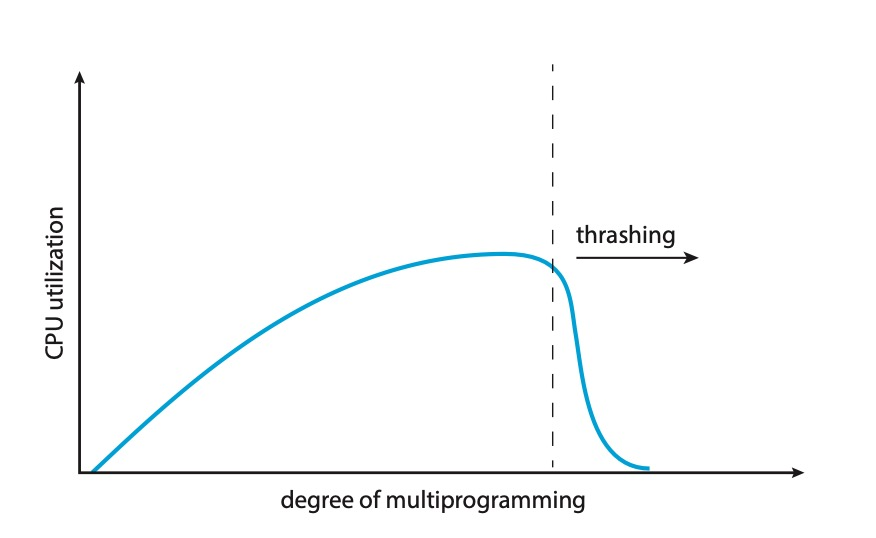
\includegraphics[width=0.4\linewidth]{assets/trashing.jpg}
\end{figure}

Vogliamo quindi trovare il massimo numero di processi che possiamo eseguire in multiprogrammazione senza incorrere nel \textit{trashing}, per decidere questo utilizziamo il modello di località.

Il modello afferma che un processo si sposta da una località ad un'altra durante la sua esecuzione, una località è un insieme di indirizzi che sono spesso utilizzati insieme.

\subsection{Working Set}
Possiamo approssimare la località di un processo guardando ai frame che esso ha utilizzato nelle ultime $\Delta$ chiamate alla memoria, chiamiamo il set dei frame usati dal processo $i$ nel periodo $\Delta$ \textit{Working Set ($WSS_i$)} .

\begin{note}
    $\Delta$ deve essere della giusta dimensione, troppo piccolo e non conterrà tutta la località, troppo grande e conterrà più località
\end{note}

Rappresentiamo il Working set con due numeri: $WS(t, \Delta)$ dove il primo è l'istante che stiamo analizzando, mentre il secondo la dimensione della località.

Otteniamo quindi $D = \sum_i WSS_i$, il numero totale di frame attualmente nella località dei processi in esecuzione, se questo numero supera il numero totale dei frame disponibili nella memoria principale si rischia di incorrere nel \textit{trashing}.

A questo punto è conveniente terminare alcuni processi o sottoporli a swapping.

\spacer
Il working set è un insieme in constante cambiamento, quindi per alleggerirne l'utilizzo è conveniente effettuare il controllo su un determinato periodo e salvare quali frame sono presenti in almeno un working set in un bit di stato (1 se presente, 0 se non presente).

Quando sarà necessario rimuovere un frame si cercherà quello con il maggior numero di 0 nei suoi bit di stato, ovvero quello che non appare nei working set da più tempo.

\subsection{Frequenza di Page Fault}
Un approccio più diretto è quello di stabilire una certa frequenza di page fault "accettabile" e aumentare o diminuire i frame di conseguenza.

\begin{figure}[H]
    \centering
    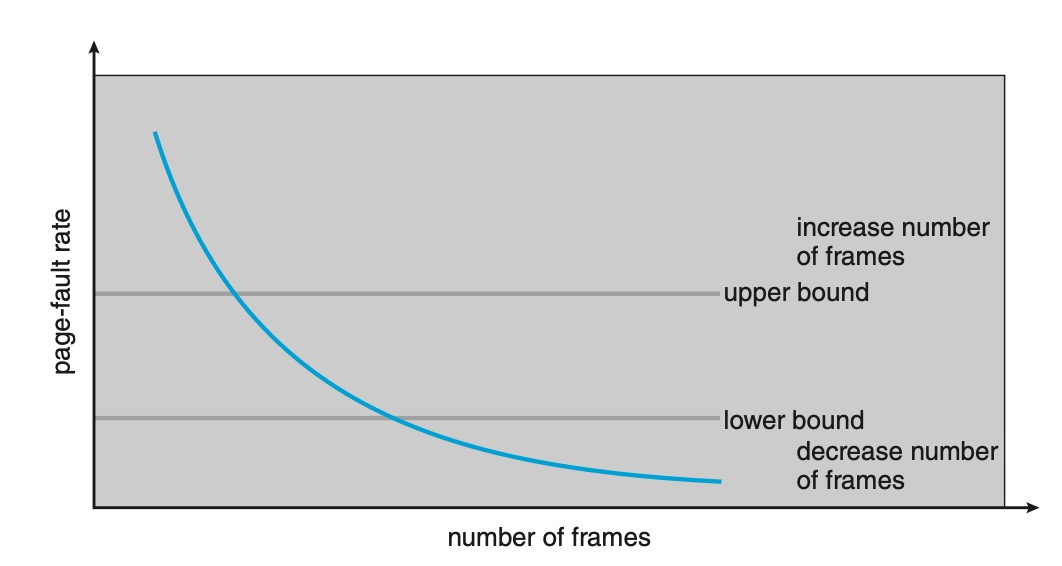
\includegraphics[width=0.5\linewidth]{assets/frequenza-page-fault.jpg}
\end{figure}

\subsection{Relazione tra Working Set e Frequenza di Page Fault}
Il cambiamento di località comporta un picco di page fault

\begin{figure}[H]
    \centering
    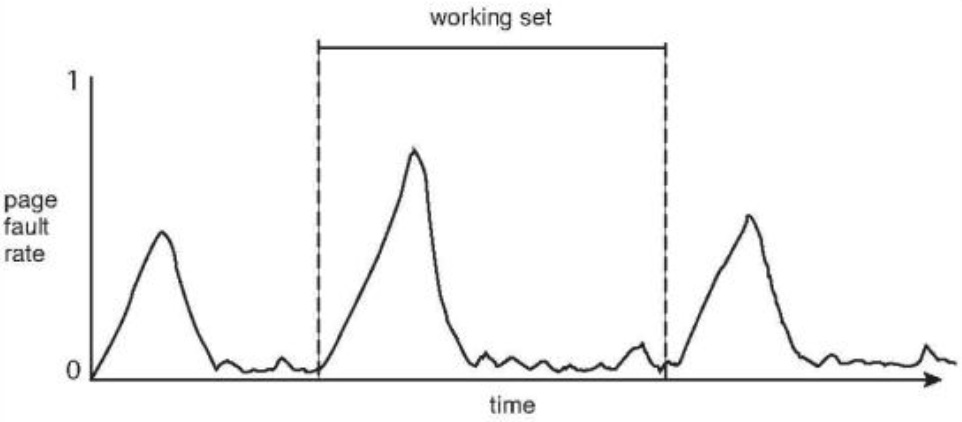
\includegraphics[width=0.5\linewidth]{assets/page-fault-working-set.jpeg}
\end{figure}
